% ----- formatovani dokumentu -----------------------------------------------
\documentclass[12pt,a4paper,titlepage,final]{report}
\usepackage[utf8]{inputenc}
\usepackage[T1, IL2]{fontenc}
\usepackage{graphicx}
\usepackage{epstopdf}
\usepackage[margin=2cm]{caption}
\usepackage[top=3cm, left=2cm, right=2cm, text={17cm, 24cm}, ignorefoot]{geometry}
\usepackage{color}
\usepackage{url}
\usepackage{setspace}
\singlespacing
\usepackage[square, numbers]{natbib} 
\pagestyle{plain}
\pagenumbering{arabic}
\setcounter{page}{1}
\setcounter{secnumdepth}{-1}
\setlength{\parindent}{1cm}	
\usepackage{natbib}
\usepackage[linesnumbered,ruled,vlined]{algorithm2e}
\SetAlgorithmName{Algoritmus}{algoritmus}

% ----- vyberte jazyk -------------------------------------------------------
\usepackage[english,czech]{babel}
%\usepackage[english]{babel}

% ----- dopiste titulky -----------------------------------------------------
\newcommand\Course{Počítačová grafika}
\newcommand\WorkTitle{Radiozita}
\newcommand\AuthorA{David Kolečkář}
\newcommand\AuthorAEmail{xkolec07@stud.fit.vutbr.cz}
\newcommand\AuthorB{Matúš Motlík}
\newcommand\AuthorBEmail{xmotli02@stud.fit.vutbr.cz}
\newcommand\Faculty{Fakulta Informačních Technologií}
\newcommand\School{Vysoké Učení Technické v Brně}
\newcommand\tab[1][1cm]{\hspace*{#1}}

\usepackage[
pdftitle={\WorkTitle},
pdfauthor={\AuthorA, \AuthorB},
bookmarks=true,
colorlinks=true,
breaklinks=true,
urlcolor=blue,
citecolor=blue,
linkcolor=blue,
unicode=true,
]
{hyperref}


% ----- titulni strana ------------------------------------------------------

\begin{document}
	\begin{titlepage}
	\begin{center}
		
\includegraphics[height=3cm]{images/logo.pdf}
	\end{center}
	\vfill
	\begin{center}
		\begin{Large}
			\Course\\
		\end{Large}
		\bigskip
		\begin{Huge}
			\WorkTitle\\
		\end{Huge}
	\end{center}
	\vfill
	\begin{center}
		\begin{large}
			\today
		\end{large}
	\end{center}
	\vfill
	\begin{flushleft}
		\begin{large}
			\begin{tabular}{lll}
				Autoři: & \AuthorA, & \url{\AuthorAEmail} \\
				        & \AuthorB, & \url{\AuthorBEmail} \\
				& & \\
				& \Faculty \\
				& \School \\
			\end{tabular}
		\end{large}
	\end{flushleft}
\end{titlepage}		
	
% ----- obsah --------------------------------------------------------------
	
\tableofcontents

% ----- zadani -------------------------------------------------------------
\newpage
\chapter{Zadání}

Cílem bylo implementovat algoritmus globální osvětlovací metody radiozity nad jednoduchou scénou vhodnou pro demonstraci tohoto algoritmu (přiměřeně složitý prostor, plošné světelné zdroje a různé materiálové vlastnosti). A nakonec zobrazit výslednou scénu pomocí knihovny OpenGL.
Radiozita je časově náročná zobrazovací metoda, která se využívá ve fotorealistické grafice. Metoda šíří světelnou energii napříč celou scénou, používá se tak k renderování 3D scén. 



%---------------------------------------------------------------------------
\chapter{Zvláštní použité znalosti}


\section{Tvorba scény}
Základem projektu bylo vytvořit scénu, na které budeme algoritmus radiozity testovat. Scénu jsme vytvářeli v 3D programu Blender. V tomto programu jsme také provedli dělení velkých ploch na menší plošky v našem případě trojúhelníky. Scénu jsme jen následně vyexportovali ve formátu \textit{.obj}, který obsahoval vrcholy a indexy trojúhelníků. Při tvorbě scény bylo důležité, aby scéna byla energeticky uzavřená a povrchy objektů byly neprůhledné. Následně jsme v našem programu naprogramovali metodu pro načítání tohoto souboru. Při jeho čtení jsme jednotlivým objektům nastavovali různé materiálové vlastnosti \cite{cite2}. 

\begin{itemize}
\item Emission barva jakou ploška vyzařuje. Hodnoty jsou omezeny od 0 do 1, přičemž 0 znamená, že povrch veškerou energii pohlcuje. V opačném případě ji odráží. 
\item Reflektivity barva kterou ploška odráží. Hodnoty jsou od 0 do 1.
\end{itemize}

\section{Konfigurační faktory}
Před výpočtem radiozity je důležité spočítat tzv. konfigurační faktory \cite{cite1} (form factors), což je vliv jedné plošky na každou jinou plošku. K výpočtu konfiguračního faktoru je nutné zobrazit scénu z pohledu cílové plošky s ploškou vyzařující světlo. A to pro každou dvojici plošek. Při tomto vykreslování stačí vidět 180$^\circ$ okolí z pohledu plošky. K tomu se využívá vykreslování do polokrychle (hemicube). Jednotlivé trojúhelníky mají ve scéně odlišnou barvu, protože je nutné jednoznačně identifikovat plošky, které jsou osvětlené ze středu polokrychle. Tudíž se index plošky zakóduje jako jeho barva a následně se pomocí Z-buffer algoritmu vypočítá, či je daná ploška viditelná ze středu polokrychle.
\begin{figure}[!b]
\begin{center}
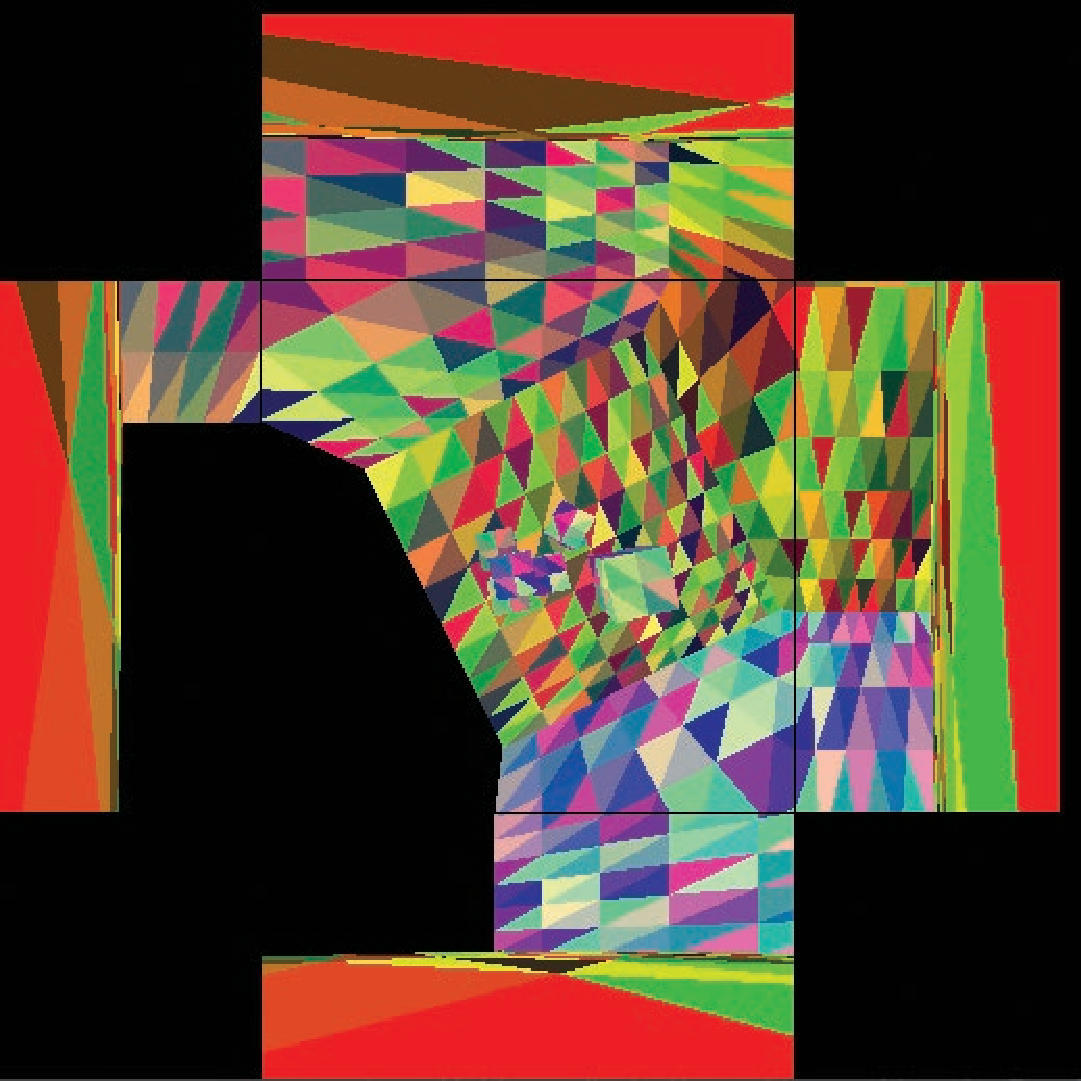
\includegraphics[height=6.1cm]{images/hemicube.pdf}
\caption{Ukázka vykreslené polokrychle.}
\end{center}
\end{figure}

Celkový konfigurační faktor (2) plošky je roven součtu tzv. delta faktorů (1) plošek na polokrychly. 
Uvedený vzorec pro výpočet delta faktoru je orientován pro horní stěnu polokrychle. Pro boční stěny je výpočet mírně odlišný. 
\begin{equation}
w_{z}(x,y) = \frac{(cos\phi_{i})^{4}}{\pi} = \frac{1}{\pi(x^{2}+y^{2}+1)^{2}}
\end{equation}

\begin{equation}
\sum_{X=-P/2}^{P/2-1}\sum_{Y=-P/2}^{P/2-1}H_{ij}(X,Y).w_{z}(X,Y)\frac{1}{P^{2}}
\end{equation}


\section{Radiozitní rovnice}

Radiozitní rovnice pro každou plošku je následující: 
\begin{equation}
B_{i} = E_{i} + R_{i} \sum_{j=1}^n B_{j}F_{ij}
\end{equation}
\begin{itemize}
\item B je radiozita dané plošky
\item E je vyzařovaná energie 
\item R je odrazivost materiálu
\item F je konfigurační faktor
\end{itemize}

\begin{algorithm}
  \SetAlgoNoLine
  \SetNlSkip{0em}
  \SetNlSty{normal}{}{:}
  \SetKwInput{Input}{Input}
  \SetKwInOut{Output}{Output}
  \SetKwFor{For}{for}{do}{to}

\Indp
  
  \textbf{for} $i = 1 $ \textbf{to} N \textbf{for} $j = 1$ \textbf{to} N \textbf{do} $F_{ij}=0$ \\
  \textbf{for} $i = 1$ \textbf{to} N \textbf{do}\\
  \tab camera = center of $\Delta$ $A_{i}$;\\
  \tab \textbf{for} k = 1 \textbf{to} 5 \textbf{ do}\\
  \tab \tab window = kth face of the hemicube;\\
  \tab \tab \textbf{for} x = 0 \textbf{to} P-1 \textbf{do}\\
  \tab \tab \tab \textbf{for} y = 0 \textbf{to} P-1 \textbf{do} pixel[x,y]=0;\\
  \tab \tab Z-BUFFER ALGORITHM (color of surface j is j)\\
  \tab \tab \textbf{for} x = 0 \textbf{to} P - 1 \textbf{do} \textbf{for} y = 0 \textbf{to} P - 1 \textbf{do} \\
  \tab \tab \tab \textbf{if}(pixel[x,y]>0) \textbf{then}\\
  \tab \tab \tab \tab $F_{i,pixel[x,y]}+=w_{k}(x-P/2,y-P/2)/P^{2};$\\
  \tab \tab \tab \textbf{endfor}\\
  \tab \tab \textbf{endfor}\\
  \tab \textbf{endfor}
        
\caption{\textsc Algoritmus počítající konfigurační faktory s využitím Z-bufferu\label{algoritmus}}
\end{algorithm}



%---------------------------------------------------------------------------
\chapter{Scéna}

Zde je zobrazena výsledná scéna, která obsahuje 1092 trojúhelníků (plošek). 
\begin{figure}[h]
\begin{center}
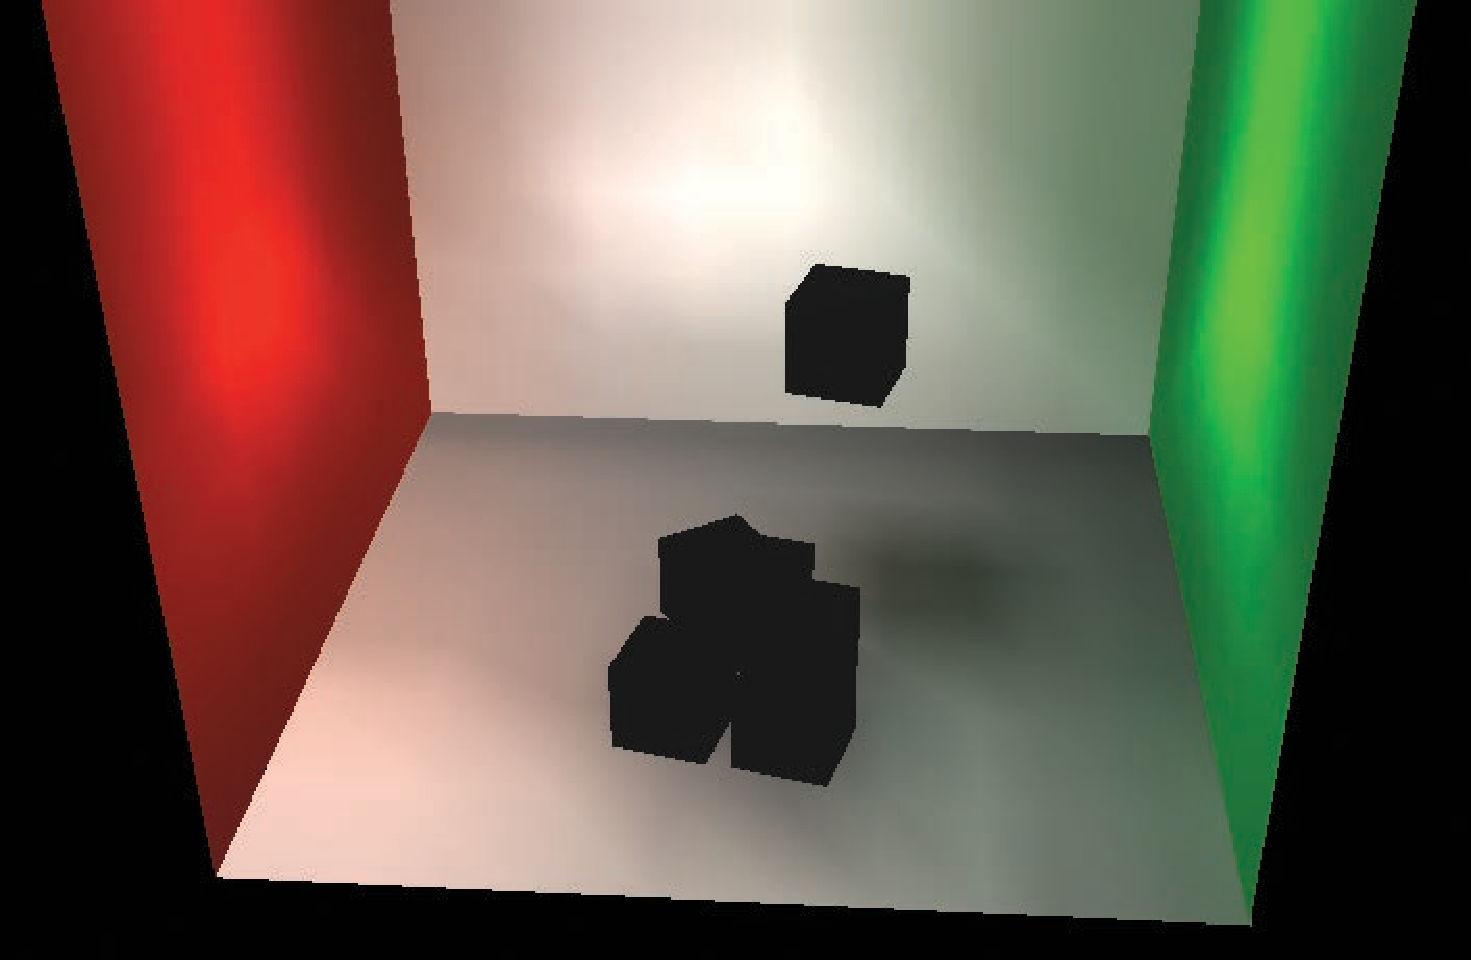
\includegraphics[height=6.9cm]{images/screenshot.pdf}
\caption{První ukázka vykreslené scény.}
\end{center}
\end{figure}

\begin{figure}[h]
\begin{center}
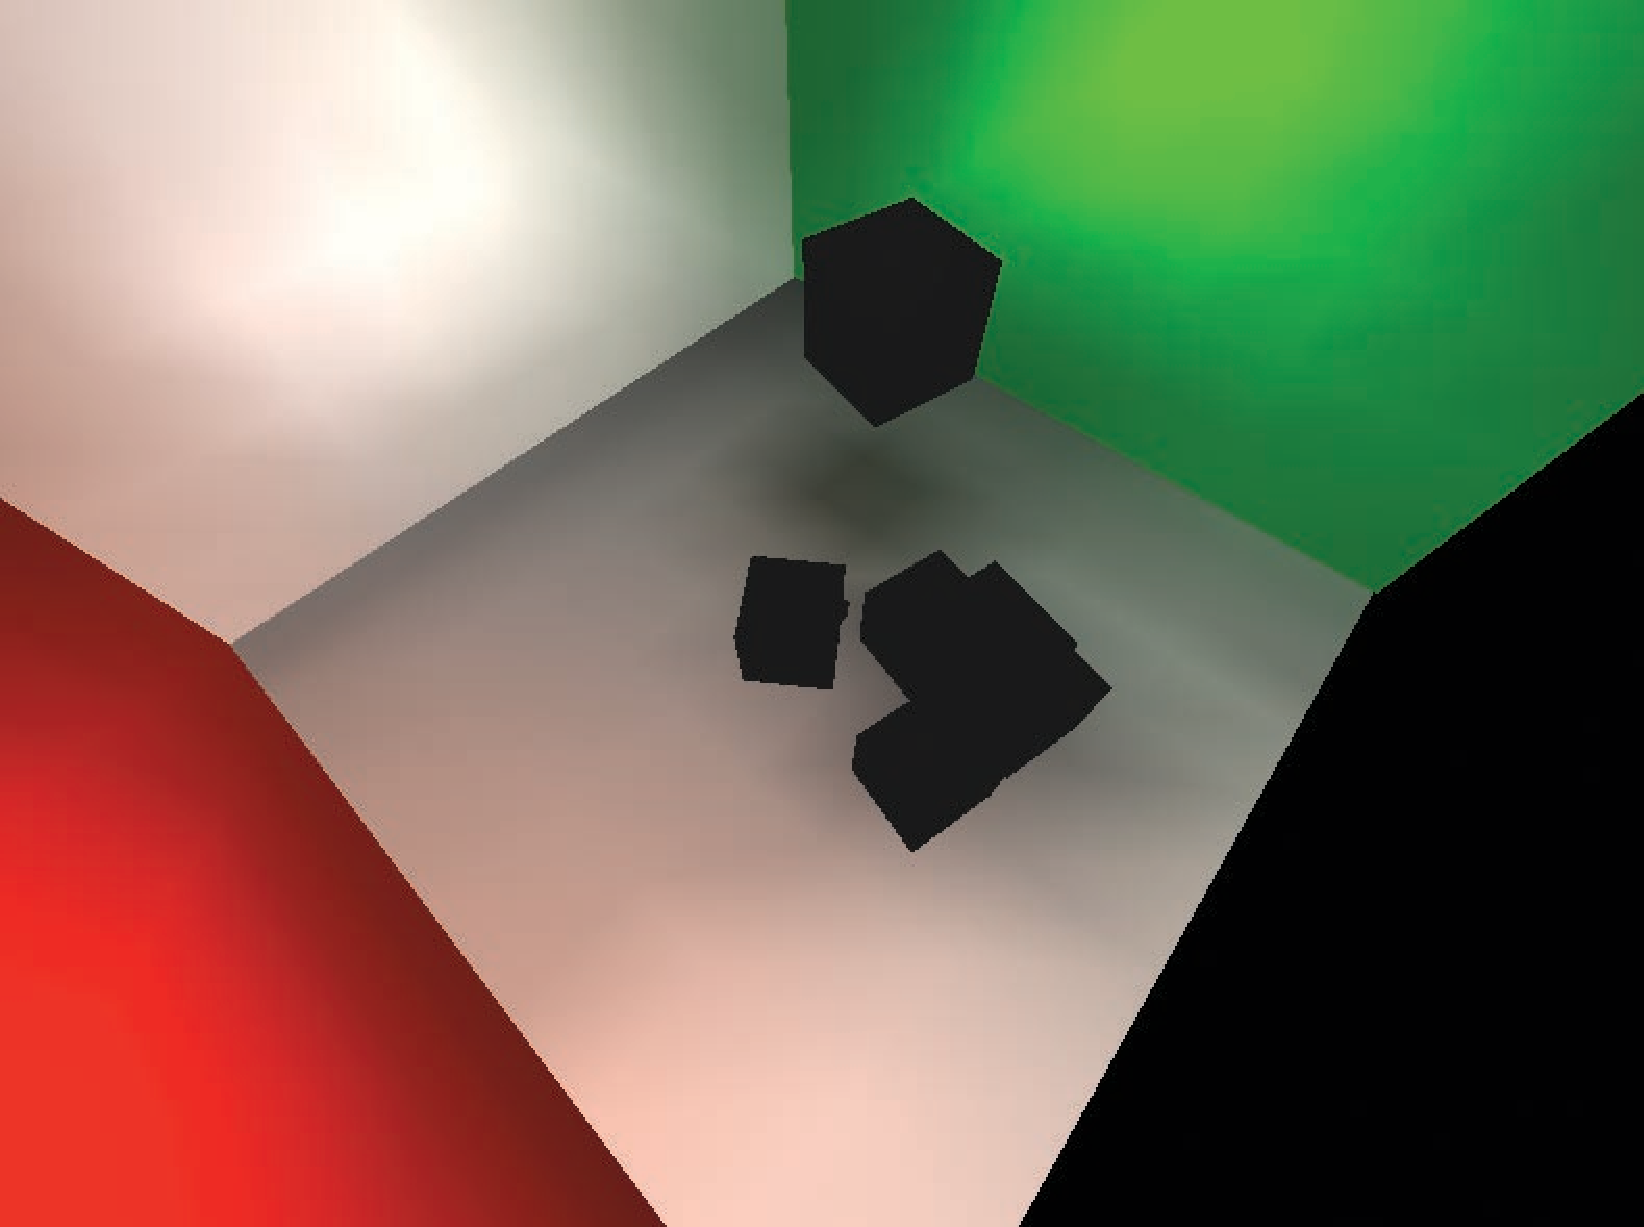
\includegraphics[height=7.7cm]{images/screenshot2.pdf}
\caption{Druhá ukázka vykreslené scény.}
\end{center}
\end{figure}

%---------------------------------------------------------------------------
\chapter{Práce na projektu}

\section{Rozdělení práce v týmu}

\begin{itemize}
\item \textbf{\AuthorA}: Vytvořena struktura programu, vytvoření scény, tvorba třídy reprezentující plošku (Triangle), dokumentace.
\item \textbf{\AuthorB}: Výpočet delta faktoru, vykreslení polokrychle, výpočet konfiguračních faktorů a vykreslení scény.
\end{itemize}

%---------------------------------------------------------------------------
\section{Co bylo nejpracnější}

Největším problémem projektu, bylo nemožnost si výsledky jednotlivých výpočtů nějak ověřit či porovnat. Při vzniklé chybě jsme tak nevěděli, zda-li je některý z výpočtů špatný či nikoliv. A celkové debugování projektu nám dělalo velký problém. 


%---------------------------------------------------------------------------
\section{Zkušenosti získané řešením projektu}

Jelikož jsme měli praktické zkušenosti s grafikou téměř nulové, byl pro nás projekt velkým přínosem. Rozšířili jsme si znalosti s programováním na GPU. Například při renderování samotné scény či polokrychle do textury. Navíc jsme si vyzkoušeli prostředí 3D programu Blender, což je profesionální nástroj na tvorbu 3D grafiky. Co se týká teoretických znalostí, tak jsme více do hloubky pochopili princip osvětlení scény a seznámili jsme se s různými metodami radiozity.

%---------------------------------------------------------------------------
\chapter{Autoevaluace}

V následujících odrážkách je uvedeno hodnocení jednotlivých částí projektu.

\paragraph{Technický návrh (75\%):} Provedli jsme vhodné rozdělení projektu na jednotlivé třídy. Program byl primárně vyvíjen pod systémem Linux, avšak mělo by být možné projekt spustit i v sytému Windows (například za pomoci Visual Studia).

\paragraph{Programování (75\%):} V kódu není mnoho komentářů, avšak vhodně pojmenované metody a proměnné přispívají k čitelnosti kódu.

\paragraph{Vzhled vytvořeného řešení (75\%):} Samotný výpočet radiozity, běží obstojně. Ovšem perfektního výsledku jsme nedosáhli z důvodu zřejmě špatné interpolace mezi jednotlivými ploškami (trojúhelníky). 

\paragraph{Využití zdrojů (80\%):} Z literatury jsme čerpali především vzorce pro výpočet delta faktoru a konfiguračních faktorů. Dále nám usnadnil práci pseudokód uvedený v \cite{cite3}.

\paragraph{Hospodaření s časem (40\%):} Projektem jsme se začali zabývat v celku brzy, avšak jen z teoretické části. Samotná implementace začala probíhat až 14 dní před odevzdáním, což se ukázalo jako velmi problematické.

\paragraph{Spolupráce v týmu (100\%):} Komunikace probíhala bez problému, většinou jsme preferovali osobní schůzky. Kód jsme sdíleli za pomoci verzovacího systému. 

\paragraph{Celkový dojem (50\%):} Z počátku zadání nevypadalo tak časově náročné jak nakonec bylo, což se projevilo na kvalitě výsledného řešení. Největším problémem bylo debugování programu. Nevěděli jsme, jak si ověřit výsledky jednotlivých výpočtů.

%---------------------------------------------------------------------------
\chapter{Ovládání vytvořeného programu}

\section{Technologie potřebné pro spuštění programu}
V následujícím seznamu jsou uvedeny knihovny, které jsou nutné pro správný běh programu.

\paragraph{OpenGL:} Vykreslování scény a polokrychle (Hemicube) probíhá za pomoci této knihovny. 

\paragraph{SDL:} Tato knihovna zajišťuje práci s okny  včetně vstupu z klávesnice a myši.

\paragraph{PGR soubor:} V projektu jsme také využili soubory pgr.c a pgr.h, které jsme používali na počítačových cvičení. Cílem těchto souborů je přiložit všechny potřebné knihovny(GLEW, GLee). Zároveň zapouzdřuje práci s knihovnou SDL. 

\paragraph{GLM:} Je matematická knihovna, zajištující práci s maticemi a vektory. 


\section{Struktura adresáře}
Zde je uvedena struktura odevzdaného adresáře. 
\begin{itemize}
\item src/ - obsahuje zdrojové kódy programu
\item doc/ - tato dokumentace ve formátu .pdf a  {\LaTeX}
\item scene/ - vykreslovaná scéna ve formátu .obj 
\item image/ - obrázky vykreslené scény pomocí radiozity
\end{itemize}

\section{Obsluha programu}
Překlad programu probíhá pomocí \textit{Makefile}, který je umístěn v adresáři se zdrojovými kódy. V tomto adresáři stačí zavolat příkaz \textit{make}, který zajistí překlad zdrojových souborů. Pro spuštění programu je zapotřebí zavolat příkaz \textit{make run}. Po spuštění programu je v okně programu zobrazena kostra scény a v příkazovém řádku vypsán počet trojúhelníků dané scény. Pro spuštění algoritmu radiozity je zapotřebí, na klávesnici stisknout klávesu \textit{r}. Pomocí myši je scénu možné různě přibližovat či rotovat. Klávesa \textit{s} umožňuje přepínat mezi scénou s radiozitou či bez ní. Lze také přepínat mezi obrysy trojúhelníků a vyplněnými trojúhelníky a to za pomoci klávesy \textit{l} respektive \textit{f}. Program lze ukončit klávesou Escape.
%---------------------------------------------------------------------------
\chapter{Doporučení pro budoucí zadávání projektů}
Projekt nakonec vyžadoval velkou časovou zátěž, ale ta plně odpovídá bodovému hodnocení. Zadání byla ponechána velká volnost, což v našem případě bylo určitě pozitivní. 



%---------------------------------------------------------------------------

\bibliographystyle{plain}

{\let\clearpage\relax\bibliography{reference}}
\addcontentsline{toc}{chapter}{Literatura}

\end{document}

